\documentclass[a4paper, 11pt]{inte}

% Faire des marges un peu moins larges que celles par défaut
\usepackage[top=20mm, bottom=20mm, left=20mm, right=20mm]{geometry}
\usepackage[utf8]{inputenc} % Pour l'encodage 
% Reconnaître les caractères accentués dans les sources.
\usepackage[T1]{fontenc} 
% Meilleurs polices
%\usepackage{concmath}
\usepackage{fourier}
\usepackage[francais]{babel}
% Insertion d'images
\usepackage{graphicx}
% Pour le listing de code
\usepackage{listings}
\usepackage{color}
% Pour fixer l'interlignage
\usepackage{setspace} 
% Pour faire un index (ici glossaire)
\usepackage{makeidx}
% Pour gérer les liens internes et les URL cliquables
\usepackage{url}
% Pour les headers et footers
\usepackage{fancyhdr}
% Pour le logo en haut a droite
\usepackage{eso-pic} 
% Pour l'enroulement du texte autour des figures
\usepackage{wrapfig}
% Pour la couverture en PDF pleine page
\usepackage{pdfpages} 
% Pour la biblio bibtex
\usepackage{bibunits}
% Pour gérer les éléments flottants
\usepackage{float}
% Pour les cadres à ombrage du glossaire
\usepackage{fancybox}
% Pour faire des sous-figures correctement numérotées
\usepackage{subfigure}
% Pour mettre les liens cliquables
\usepackage{hyperref}
\usepackage{lettrine}
\usepackage{multicol}
\usepackage{rotating}
\usepackage{amsmath}
\usepackage{cclicenses}
%headers, footers
\pagestyle{fancy}
\rhead{INSA de Lyon}
\lhead{Poly d'inté IF'2010}
\cfoot{\thepage}
\renewcommand{\footrulewidth}{0.4pt}

% Séparation entre les deux colonnes
\setlength{\columnsep}{0.8cm}
% Largeur de la ligne de séparation
%\setlength{\columnseprule}{1pt}

% Changer la fonte vers Helvetica
%\usepackage{helvet}
% Changer la fonte vers Libris ADF
%\usepackage{libris}
% Changer la fonte vers Venturis Sans
\usepackage[lf]{venturis}

% Pour mettre en sans-serif par défaut
\renewcommand*\familydefault{\sfdefault} 
% Unité pour pstricks
\setlength{\unitlength}{1mm}

%\AddToShipoutPicture{%
%\setlength{\unitlength}{1mm}%
%\put(20, 10){%
%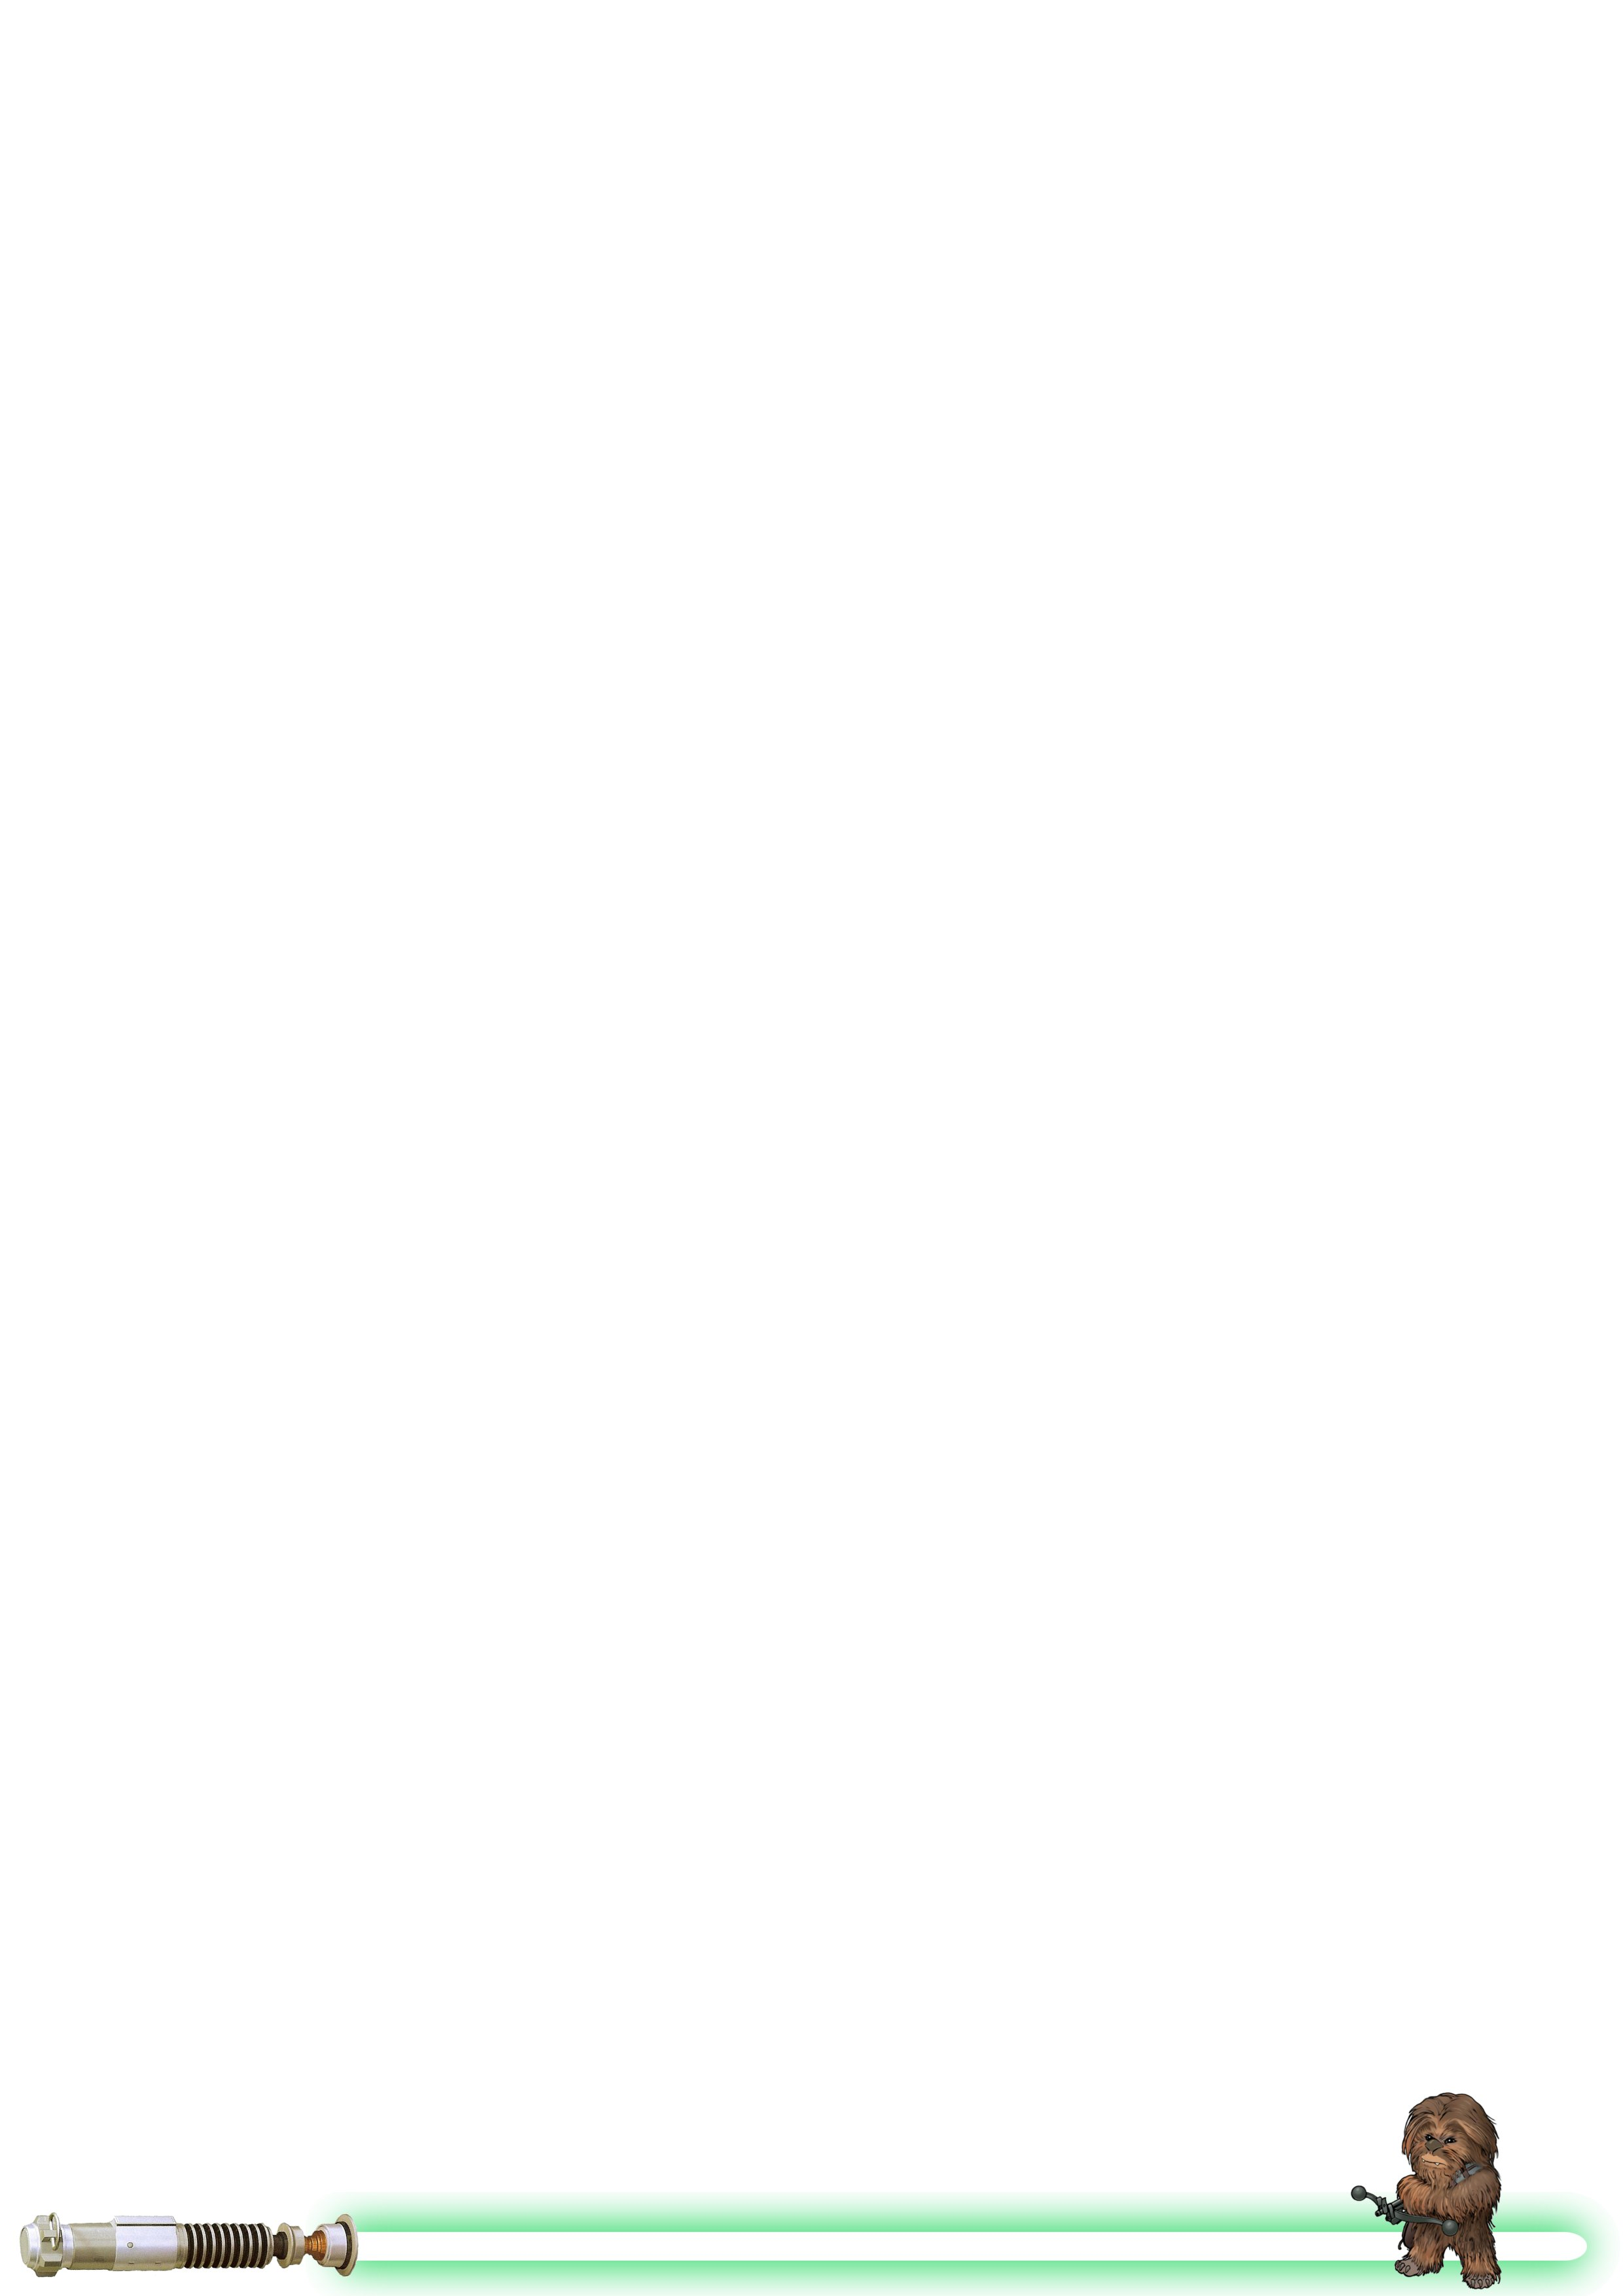
\includegraphics[width=\textwidth]{images/footer.png}}}

% Couleur des url et des liens internes.

\definecolor{sectionColor}{rgb}{0,0,1}
\definecolor{subSectionColor}{rgb}{0,0,0.8}
\definecolor{subSubSectionColor}{rgb}{0,0,0.6}
\definecolor{coulcitation}{rgb}{0.90,0.90,0.90}
\definecolor{bleuLien}{rgb}{0, 0, 0.8}
\setlength{\headheight}{13.6pt}


\hypersetup{
    pdftitle={Poly d'inté IF'2010},    % title
    pdfauthor={Équipe d'inté IF'2010},     % author
    pdfsubject={On peut mettre plein de trucs ici. Alors la recette de la 	tarte à la rhubarbe : Pour 6 personne(s) -Pour la pate sablée : 300 g de farine, 2 cuillères à soupe d'huile, 2 cuillères à soupe de lait, 2 cuillères à soupe de sucre, 125 g de beurre mou, 1 jaune d'oeuf(conserver le blanc pour la crème) -Pour la garniture : une belle botte de rhubarbe pelée et coupée en gros dés , 2 cuillères à soupe de crème fraiche épaisse, 2 oeufs et le blanc restant, 125 g de sucre, un peu de lait ,1 cuillère à café de maïzena PREPARATION 1 Mélanger la farine, le sucre, le beurre ramolli, ajouter le jaune d'oeuf , l'huile et le lait. Malaxer, bien rajouter un peu de farine si nécessaire pour que la pâte ne colle plus aux doigts.  2 Placer la boule de pâte au frais, 1 heure environ.  3 Etaler la pate à la main dans un moule à manqué avec revêtement anti adhésif.  Disposer les tronçons de rhubarbe sur la pâte.  4 Dans un saladier, battre les oeufs plus le blanc avec le sucre, ajouter la maïzena, puis le lait et la crème en mélangeant bien. Garnir la tarte.  5 Cuire au four préchauffé à 225°C pendant 30 à 40 minutes, la crème ne doit plus être liquide.  6 La démouler une fois refroidie est risqué mais possible en utilisant 2 plats à tarte.  },   % subject of the document
    pdfkeywords={IF Inté 2010 -- Martius est un usurpateur qui n'a rien à faire là --. Oh, mais là aussi on peut marquer plein de truc. Alors si tu vois ça, tu peux envoyer un mail à l'équipe d'inté, ça nous fera plaisir d'être soutenu dans notre stupidité : \texttt{bonjourlesifs@gmail.com}.  Allez, à plus, et merci pour tout le poisson.}, % list of keywords
    colorlinks=true,
    linkcolor=bleuLien,          % color of internal links
    urlcolor=bleuLien, % color of external links
    linkbordercolor=bleuLien
}



\renewcommand{\LettrineFontHook}{\fontfamily{pag}%
                \fontseries{bx}\fontshape{it}\color{red}}

  \newenvironment{changemargin}[2]%
  {\begin{list}{}{%
    \setlength{\listparindent}{\parindent}%
    \setlength{\itemindent}{\parindent}%
    \setlength{\leftmargin}{#1}%
    \setlength{\rightmargin}{#2}%
  }\item }%
{\end{list}}


% Boites pour citation
\newsavebox{\auteurcitation}
\newsavebox{\boitecitation}
\newenvironment{citationi}[1]
{% 
    \savebox{\auteurcitation}{#1}
    \begin{lrbox}{\boitecitation}
    \begin{minipage}{.8\linewidth}
    \small \slshape «~\ignorespaces
}
{%
    \unskip{}~»  

    \par\nopagebreak\hfill\usebox{\auteurcitation}

    \end{minipage}
    \end{lrbox}

    \begin{center}
	\colorbox{coulcitation}{\usebox{\boitecitation}}
    \end{center}
}

\newenvironment{citationii}[1]
{% 
    \begin{lrbox}{\boitecitation}
    \begin{minipage}{.8\linewidth}
    \small \slshape «~\ignorespaces
}
{%
    \unskip{}~»  

    \end{minipage}
    \end{lrbox}

    \begin{center}
	\colorbox{coulcitation}{\usebox{\boitecitation}}
    \end{center}
}

\newcommand{\carre}[2]{%
\begin{center}
\begin{picture}(#1,#2)
    \framebox(#1,#2){}
\end{picture}
\end{center}
}

\newcommand{\orga}[1]{%
\begin{center}
	\includegraphics[height=5cm]{#1}%
\end{center}
}




\newcommand{\adresseCoupon}{%
\begin{center}
\colorbox{coulcitation}{
    \begin{minipage}{.8\linewidth}
	M\up{elle} Sandra \textsc{Mondain}\\
	Appartement 13 \\
	130, rue du 4 août 1789 \\
	69100 Villeurbanne 
    \end{minipage}
}
\end{center}%
}

\newcommand{\plex}[2]{%
    \vspace{0.3em}
    \shadowbox{#1} \\
    #2

}


